\subsection{Quantum Monte Carlo Simulations\label{sec:MC_quanten}
In the quantum field three problems has to be solved. (\cite{1905.02666})
\begin{enumerate}
	\item Load the probability Estimation (the log-normal distribution) in to the quantum computer. This problem is described in section \ref{sec:MC_QGAN}
	\item The payoff function $F(\textbf{X})$ has to be build with qubits inside the quantum computer. In section \ref{sec:MC_Payoff} the payoff function is constructed.
	\item The quantum computer should calculate at the end the expected value of the payoff $\mathbb{E}_P[F(\textbf{X})]$, this will also be explained in section \ref{sec:MC_Payoff}.
\end{enumerate}
But before we can describe how to construct the gates to build the payoff function, we need to explain how amplitude estimation is working in an quantum computer. We are doing this in section \ref{sec:MC_AE}

\subsubsection{Loading the distribution (QuGAN)}\label{sec:MC_QGAN}
In this section we go over the basics of the QuGAN, because we use an already implemented function, which is not QuGAN, of qiskit (\cite{Qiskit}) later to load in the log-normal distribution.

QuGAN stands for Quantum Generative Adversarial Networks and it creates fake data which are similar to the real data. The GAN method is used when there are only a few real world data or to bring the data in to a new system. The last one is exactly our purpose here. We want to have the log-normal distribution inside a quantum computer. For this we divide the log-normal distribution in distinct buckets $n$. The value of $n$ has to be the number of states the $k$ qubits can have $n=2^{k}$. So if we have 3 qubits we have 8 distinct buckets. Every state of all the $k$ qubits maps to a real value.

The structure of an QuGAN is shown in figure \ref{fig:qgan}. So a QuGAN goes throw this steps:
\begin{enumerate}
	\item We load in at first the classical dataset, transform the Dateset and with this dataset initial parameter for the gates can be created.
	\item With this parameters the quantum circuit can be created. \label{enu:QuGan_parameter}
	\item The quantum circuit is then loaded into a quantum computer.
	\item After optimise steps in the quantum computer the quantum state is measured.
	\item The quantum state is then transformed in to the classical world and the loss is calculated. Also the Quantum Circuits can create sample states and this sample states are then used to generate classical data points.
	\item With the loss the parameters of the circuit can be update. After updating the circuits parameter we go back to step \ref{enu:QuGan_parameter}.
\end{enumerate}
\begin{figure}[H]
  \begin{center}
    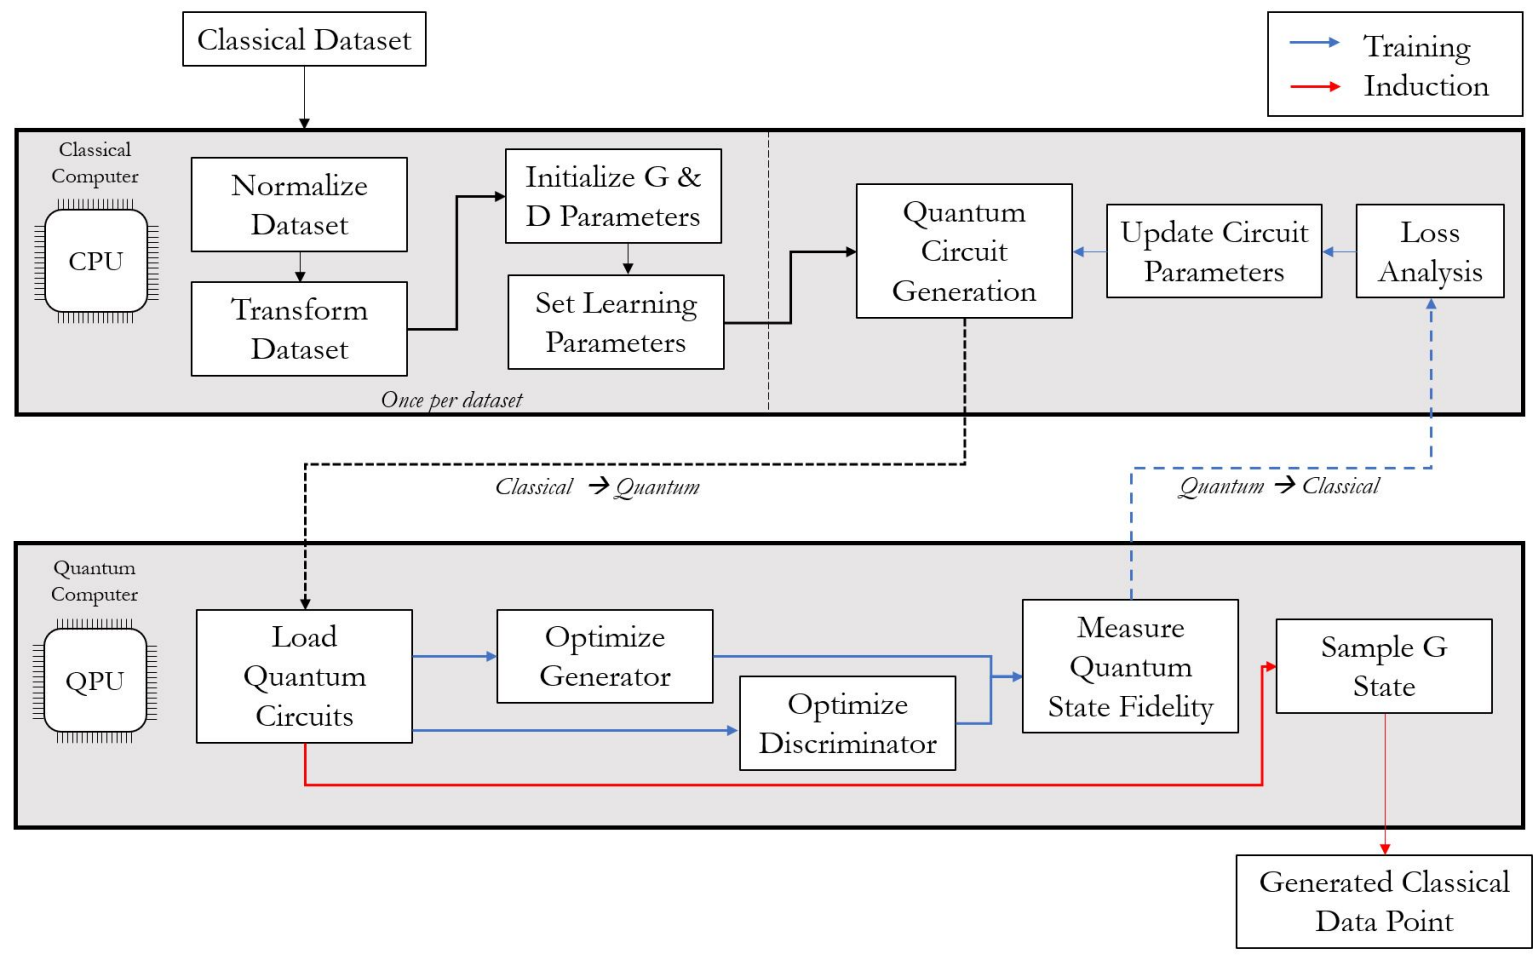
\includegraphics[width=\linewidth]{images/qgan_structure.png}
  \end{center}
  \caption{ QuGAN System Architecture \cite{2010.09036}}
  \label{fig:qgan}
\end{figure}
\subsubsection{Amplitude Estimation}\label{sec:MC_AE}
For the Amplitude Estimation (AE) we need an unitary operator $A$ which behaves on an register of $(n+1)$ qubits like this
\begin{align}
    A\ket{0}_{n+1} &= \sqrt{1-a}\ket{\psi_0}_{n}\ket{0}+\sqrt{a}\ket{\psi_1}_{n}\ket{1}. \label{eq:AE_A}
\end{align}

In the equation \ref{eq:AE_A} $\ket{\psi_0}_{n}$ and $\ket{\psi_1}_{n}$ are some normalized states and $a$ is a unknown variable $\in [0,1]$.
With Amplitude Estimation we can estimate the value of $a$ therefor we have to construct our problem so that we have this at the end $a=\mathbb{E}_P[f(\textbf{X})]$.
To make a use of $\sin$ and $\cos$ to work with RY-Gates we can say that $a=\sin^2(\theta_a)$ is, so that equation \ref{eq:AE_A} turns into this
\begin{align}
    A\ket{0}_{n+1} &= \cos(\theta_a)\ket{\psi_0}_{n}\ket{0}+\sin(\theta_a)\ket{\psi_1}_{n}\ket{1}. \label{eq:AE_A_sin} \\
    \theta_p &= 2 \theta_a \nonumber \\
    A &= R_Y(\theta_p)
\end{align}

With this changes we transformed the amplitude estimation in to a phase estimation.\\
The next step is to determine the Grover operator $\mathcal{Q}=AS_0A^\dagger S_{\psi_1}$.\\
$S_0$ is a reflection about the $\ket{0}$ state and $S_{\psi_1}$ is a reflection about the $|\psi_1>$ state. So we can write $S$ and $\mathcal{Q}$ like this:
\begin{align}
    S_0 &= 1-2\ket{0}\bra{0} \nonumber \\
    S_{\psi_1} &= 1-2\ket{\psi_1}\ket{0}\bra{\psi_1}\bra{0} \nonumber \\
    \mathcal{Q} &= R_Y(2\theta_p) \\ 
    \mathcal{Q}_{2^j} &= R_Y(2^j\cdot 2\theta_p)
\end{align}
\begin{figure}[H]
  \begin{center}
\begin{quantikz}
\lstick{(0) \ket{0}} & \gate{H} & \ctrl{5} & \ldots \qw & \qw & \ldots \qw & \qw & \gate[5, nwires={2,4}]{QFT^{\dagger}} &  \meter{}\\
 & \vdots & & \ddots & & \ddots & & \\
\lstick{(j) \ket{0}} & \gate{H} & \qw & \ldots \qw & \ctrl{3} & \ldots \qw & \qw & & \meter{}\\
 & \vdots & & \ddots & & \ddots & &\\
\lstick{(n-1) \ket{0}} & \gate{H} & \qw & \ldots \qw & \qw & \ldots \qw & \ctrl{1} & &  \meter{}\\
\lstick{(n) \ket{0}} & \gate[wires=2]{A} & \gate[wires=2]{\mathcal{Q}_{2^0}} & \ldots \qw & \gate[wires=2]{\mathcal{Q}_{2^j}} & \ldots \qw & \gate[wires=2]{\mathcal{Q}_{2^{n-1}}} & \qw\\
\lstick{(n+m-1) \ket{0}} &  & & \ldots \qw &  & \ldots \qw & & \qw
\end{quantikz}
\end{center}
\caption{ Design of the Amplitude Estimation recreated after \cite{1905.02666}}
\label{fig:qgan}
\end{figure}
The error $\epsilon$ of this method defined as followed
\begin{align}
    |\hat{\Pi} - \Pi| &\leq C\cdot(\frac{\sqrt{\mathbb{E}}}{M} + \frac{1}{M^2}) \nonumber \\
    M &= \mathcal{O}(\frac{1}{\epsilon \sqrt{\mathbb{E}}}) \label{eq:AE_M}
\end{align}
As we can see in \ref{eq:classic_M} and \ref{eq:AE_M} quantum computer improved the number error with the same number of samples
\subsubsection{Construct the payoff function}\label{sec:MC_Payoff}
A lot of payoff function can be constructed by piece-wise linear functions, in this section we will go over how to construct the piece-wise linear function in to quantum computer.

First of all we need to transform the payoff function $F(\textbf{X})$ in to new functions $f_b(i)=m_b\cdot i + o_b$, with $m_b$ the slope of the function and $o_b$ the offset of the function. For every break point $b$ of the payoff function we need to create a new function $f_b$. The new function gets the following as input $i\in\{0,\ldots, 2^n-1\}$, which represents all states the qubits can have. For example we have three qubits ($i\in\{0,1,2,3,4,5,6,7\}$) so $\ket{011}$ mapes to $i=3$. The output of the function can also only be $f(i)\in[0,1]$ this was shown in section \ref{sec:MC_AE}. Now that we build the function we can insert the function in this equation \ref{eq:AE_A_sin} and get this new equation
\begin{align}
    \ket{i}_n\ket{0} &= \ket{i}_n(\cos[f(i)]\ket{0}+\sin[f(i)]\ket{1}) \label{eq:PF_f}
\end{align}

So this function can be rebuild in a quantum computer with controlled $Y$-Rotations $CR_y$ and normal $Y$-Rotations $R_y$, the normal $Y$-Rotation is only used to initially rotate the qubit, which corresponds to the first offset. To do this we need an extra qubit on which we perform the rotations based on $x$ encoded in register $\ket{i}_n$ which is already holding the probability distribution. Similar to the Amplitude Estimation the rotations add a factor $2^{j}$, where the ${j}$'s are qubits from $\ket{i}_n$-register. (shown in figure \ref{fig:PF_y}) Consequently the more $\ket{j}$ are set to $\ket{1}$, the higher the value of $x$ is. If we add more qubits to $\ket{i}_n$-register, i.e. more grid-points, a higher accuracy can be reached.

\begin{figure}[H]
  \begin{center}
\begin{quantikz}
\lstick{\ket{q_0}} & \qw & \ctrl{3} & \qw & \qw & \qw\\
\lstick{\ket{q_1}} & \qw & \qw & \ctrl{2} & \qw & \qw\\
\lstick{\ket{q_2}} & \qw & \qw & \qw & \ctrl{1} & \qw\\
\lstick{\ket{q_3}} & \gate[1]{R_y(f_0)} & \gate[1]{CR_y(f_1)} & \gate[1]{2CR_y(f_1)} & \gate[1]{4CR_y(f_1)} & \qw
\end{quantikz}
\end{center}
\caption{ Quantum circuit for a linear function. Base image copied from \cite{1905.02666}}
\label{fig:PF_y}
\end{figure}

Until now we only showed how to implement a linear function but every piece-wise linear function applies only on specific states. Now we have to build a greater or equal operation in a quantum computer, since we are dealing with a $max$ function in eq. $\ref{eq:E_example_european}$. For this we need also $n$ qubits, one of the qubits has the result at the end. So for this operation we have $n$ data qubits $\ket{q}$ and $n$ qubits for the greater or equal operation $\ket{a}$. To build the operation we can follow this steps (example of a circuit is in figure \ref{fig:PF_max}). 
\begin{enumerate}
	\item At first we convert the breakpoint $b\in[0,2^n-1]$ in a bit representation $t$. For this we use a ceil operation on b and convert it then in a bit representation $t$. Every bit represent one qubit. If the breakpoint lies between two grid points $i$, the ceil operation ensures that the respective larger grid point is used as breakpoint for controlled application of max-operation.
	\item Now we can iterate over all the qubits. (we use here $j$ as iterate parameter)
	\begin{itemize}
	    \item if it is the first qubit $j=0$ and $t[j]=1$, we have to perform a $CX$ operation on $\ket{q_j}$ and $\ket{a_j}$.
	    \item if $t[j]=1$ an $OR$-Operation has to be done on $\ket{q_j}$ and $\ket{a_{j-1}}$ the result of the $OR$-Operation will be saved in $\ket{a_j}$
	    \item if $t[j]=0$ an $CCX$-Operation has to be done on $\ket{q_j}$, $\ket{a_{j-1}}$ and $\ket{a_j}$
    \end{itemize}
    \item Now we have in $a_{n-1}$ the result saved $\ket{0}$ if $i<b$ and $\ket{1}$ if $i\geq b$.
    \item What we have to do now is to reverse the process except that now $j\in{n-1, \ldots, 0}$ is. So we do not consider the last qubit because it saves the result. To reverse an $CX$, $CCX$ and $OR$-Operation we only have to apply the same operator again.
\end{enumerate}
\begin{figure}[H]
  \begin{center}
\begin{quantikz}
\lstick{\ket{a}} & \gate{X} & \ctrl{2} & \gate{X} &  \midstick[3,brackets=none]{$\equiv$}\qw & \ctrl{2} & \qw\\
\lstick{\ket{b}} & \gate{X} & \ctrl{1} & \gate{X} & \qw & \ctrl{1} & \qw\\
\lstick{\ket{c}} & \gate{X} &  \targ{} & \qw & \qw & \gate{OR} & \qw
\end{quantikz}
\end{center}
\caption{ Example of an $OR$-Operation on qubit $\ket{a}$ and $\ket{b}$. The result is then saved in $\ket{c}$. Base image copied from \cite{1905.02666}}
\label{fig:PF_OR}
\end{figure}

\begin{figure}[H]
  \begin{center}
\begin{quantikz}
 & & & & &  & & & & & & &  \gategroup[9,steps=7,style={dashed,rounded corners,fill=blue!20, inner xsep=2pt},background]{{Inverse for n-2 to 0}}    & & & &  &  &    \\
\lstick{\ket{q_0}} & \ctrl{4}\gategroup[5,steps=1,style={dashed,rounded corners, inner xsep=2pt}]{{t[0]=1}} & \qw & \qw & \qw & \qw & \qw  & \qw & \qw & \qw & \qw & \qw & \qw & \qw & \qw & \qw & \qw & \ctrl{4}\gategroup[5,steps=1,style={dashed,rounded corners, inner xsep=2pt}]{{t[0]=1}} & \qw  \\
\lstick{\ket{q_1}} & \qw & \qw & \ctrl{4}\gategroup[5,steps=1,style={dashed,rounded corners, inner xsep=2pt}, label style={label position=below,anchor=north,yshift=-0.2cm}]{{t[1]=0}} & \qw & \ctrl{4}\gategroup[5,steps=1,style={dashed,rounded corners, inner xsep=2pt}, label style={label position=below,anchor=north,yshift=-0.2cm}]{{t[1]=1}} & \qw & \qw & \qw & \qw & \qw & \qw & \qw & \ctrl{4}\gategroup[5,steps=1,style={dashed,rounded corners, inner xsep=2pt}, label style={label position=below,anchor=north,yshift=-0.2cm}]{{t[1]=0}} & \qw & \ctrl{4}\gategroup[5,steps=1,style={dashed,rounded corners, inner xsep=2pt}, label style={label position=below,anchor=north,yshift=-0.2cm}]{{t[1]=1}} & \qw & \qw & \qw \\
\lstick{\vdots} & & & &  & & \vdots & & & & & \vdots & & & & &  &  &    \\
\lstick{\ket{q_{n-1}}} & \qw & \qw & \qw & \qw & \qw & \qw & \qw & \ctrl{4}\gategroup[6,steps=1,style={dashed,rounded corners, inner xsep=2pt}]{{t[n-1]=0}} & \qw & \ctrl{4}\gategroup[6,steps=1,style={dashed,rounded corners, inner xsep=2pt}]{{t[n-1]=1}} & \qw & \qw & \qw & \qw & \qw & \qw & \qw & \qw \\
\lstick{\ket{a_0}} & \targ{} & \qw & \ctrl{1} & \qw & \ctrl{1} & \qw & \qw & \qw & \qw & \qw  & \qw & \qw & \qw & \qw & \qw & \qw & \targ{} & \qw   \\
\lstick{\ket{a_1}} & \qw & \qw & \targ{} & \qw & \gate{OR} & \qw & \qw & \qw & \qw & \qw & \qw & \qw & \targ{} & \qw & \gate[style={fill=blue!20}]{OR} & \qw & \qw & \qw \\
\lstick{\vdots} & & & & & & \vdots & & & & & \vdots & & & &  & &  & \\
\lstick{\ket{a_{n-2}}} & \qw & \qw & \qw & \qw & \qw & \qw & \qw & \ctrl{1} & \qw & \ctrl{1} & \qw & \qw & \qw & \qw & \qw & \qw & \qw & \qw \\
\lstick{\ket{a_{n-1}}} & \qw & \qw & \qw & \qw & \qw & \qw & \qw & \targ{} & \qw & \gate{OR} & \qw & \qw & \qw & \qw & \qw  & \qw & \qw & \qw 
\end{quantikz}
\end{center}
\caption{ Basic structure of an circuit for the bigger then operation. Base image copied from \cite{1905.02666}}
\label{fig:PF_max}
\end{figure}

So now we have a qubit $a_{n-1}$ (control qubit) which holds the information if $i\geq b$. This control qubit is then used to control if the rotations of breakpoint $b$ are executed or not. After applying the $Y$ Rotations for a breakpoint $b$ the inverse of the greater or equal operation has to applied to the circuit, so that the states are all $\ket{0}$ for the next breakpoint. 
Note that a smaller-than operations can be realized by adding a bit-flip X-gate to qubit $a_{n-1}$.
\\   

Now that we have shown how to construct a piece-wise linear function in a quantum computer we change $\theta_P$ again to better obtain our desired result $\mathbb{E}$.
\begin{align}
    \theta_P &= c\tilde{f}_b(i)+\frac{\pi}{4}\label{eq:theata_P} \\
    \tilde{f}_b(i) &= 2 \frac{f_b(i)-f_{\text{min}_b}}{f_{\text{max}_b}-f_{\text{min}_b}}\label{eq:f_bi}
\end{align}

Equation \ref{eq:theata_P} is chosen to center $ \sin^2(\theta_P) $ around $\tilde{f}_b(i) = 0$ and \ref{eq:f_bi} so that $\tilde{f}_b(i) \in [-1,1] $

At the end of the Amplitude Estimation we only have to calculate the result.
To obtain an approximation for $\tetha_p$, AE applies Quantum Phase Estimation to approximate certain eigenvalues of \mathcal{Q}, which are classically mapped to an estimator for $a$. The Quantum Phase Estimation uses $m$ additional sampling qubits to represent result and $M = 2^m$ applications of $\mathcal{Q}$, i.e., $M$ quantum samples. The m qubits, initialized to an equal superposition state by Hadamard gates, are used to control different powers of $\mathcal{Q}$. After applying an inverse Quantum Fourier Transform, their state is measured resulting in an integer $y \in \{0, ..., M − 1\}$, which is classically mapped to the estimator for a, i.e.
\begin{equation}
    \tilde{a} = \sin^2(y \pi / M) \in [0,1] \label{eq:estimate_a}.
\end{equation}
\bibliography{././refs}